\documentclass{article}
\usepackage[utf8]{inputenc}
\usepackage{kotex}
\usepackage{color}
\usepackage{fancyhdr}
\usepackage{geometry}
\geometry{
    a4paper,
    total={170mm,257mm},
    left=20mm,
    top=20mm,
}

\lhead{\large 2022년 봄 POSTECH 컴퓨터공학과 과제연구 연구계획서\\[1.3cm]}
%\lhead{\parbox[][\headheight][t]{2cm}{\textbf{Citation:}}}
%\rhead{\parbox[][\headheight][b]{2cm}{\raggedleft Page\,\thepage{} of \pageref{LastPage}}}
\rhead{
\includegraphics[width=2.5cm]{logo}}
\renewcommand{\headrulewidth}{0pt}
%\title{[제목]\hfill
\includegraphics[width=2cm]{logo}}
\title{MOTD: Modular Two-pass Defense Network without Vaccination against Adversarial Example}
\author{이름: 권민재\\학번: 20190084\\연구지도교수: 김종}


\date{2022. 3. 10.}

\usepackage{natbib}
\usepackage{graphicx}




\begin{document}
\maketitle\thispagestyle{fancy}

\noindent\makebox[\linewidth]{\rule{\textwidth}{0.4pt}}

\section{연구 목적}
%연구의 주제를 서술하고 그 중요성과 필요성을 설명합니다.

최근 인공신경망을 이용한 이미지 분류는 단순히 이론적인 수준을 넘어 사람들이 많이 사용하는 여러 서비스들에 공격적으로 도입되고 있다. 예를 들어, 온라인 사진 앨범 서비스들이 사진들에 포함된 얼굴을 분류해주는 기능을 소비자에게 제공하는 것을 넘어, 자율주행차가 카메라를 통해 실시간으로 사물을 인식하고 분류하는 데에도 인공 신경망이 이용되고 있다. 이러한 classifier들이 여러 서비스와 연구의 밑바탕으로 활약하고 있는 것과 달리, 최근 연구들은 classifier들을 속일 수 있는 여러 공격 기법들을 보여주고 있다. FSGM (Fast Gradient Signed Method), PGD (Projected Gradient Descent) 등의 공격 방법을 시효로 이미지 분류 인공 신경망에 대해 다양한 공격 방법이 연구 및 제시되었다. 특정 신경망에 대한 adversarial example을 생성하는 공격 방법이 주를 이뤘으며, 이에 대한 방어 방법 또한 지속적으로 소개되고 있다.

Adversarial example에 대한 방어법은 크게 세 가지 정도로 분류해볼 수 있다. \textbf{(1)} 첫번째로, adversarial example들을 인공 신경망에 직접 학습시키거나, adversarial example을 분류해낼 수 있도록 학습시키는 방법이 존재한다. 하지만 adversarial example을 직접 이용하는 방식에는 분명한 한계점이 존재한다. 종래의 adversarial attack들은 그 각각의 공격 방법에 따라 매우 다양한 형태의 example들을 생성한다. 이들을 모두 수집하여 예외적으로 인공 신경망에 학습시키는 것은 현실적으로 불가능하다고 판단되기 때문에, 효율적인 방어를 해낼 수 없다. \textbf{(2)} 둘째로, 임의의 분류기를 통해 인공 신경망에 입력되는 이미지를 사전에 분류하는 방법이 존재한다. Adversarial example 인지 아닌지를 구별할 수 있는 장치를 통해 인공 신경망에 adversarial example이 입력되지 않도록 방어하는 것이다. 예를 들어, \textbf{MagNet}은 autoencoder 형태의 detector를 통해 이와 같은 관점을 일부 채택하였다. 하지만 이러한 방법은 adversarial example에 대해 인공 신경망이 올바른 판단을 내리도록 도움을 주는 방향이 아닌, 해당 이미지에 대한 판단을 내리지 않도록 만드는 것이기에 classifier의 기능성을 저해시키는 요인으로 작용한다는 점이 부족하다고 말할 수 있다. \textbf{(3)} 마지막으로, 인공 신경망에 입력되는 이미지를 전처리하는 방법이 존재한다. 전처리를 통해 이미지에 임의로 삽입된 정보들을 상쇄시켜 example의 perturbation을 줄이는 관점이다. 하지만 이미지를 직접 수정하는 만큼 오히려 classifier를 방해할 수 있다는 지적이 나오고 있다. 예를 들어, \textbf{SHIELD}는 이미지 전처리를 이용하는 대표적인 방어법이다. \textbf{SHIELD}는 JPEG compression를 통해 불필요한 정보를 제거하여 방어를 수행하지만, compression 과정이 분류 체계를 방해하지 않도록 기존 신경망을 "vaccinate" 해야만 했다. \cite{das2018shield} 즉, 이미지에 대한 전처리 과정이 인공 신경망을 방해할 뿐만 아니라 방어 시스템 도입의 이식성을 저해하고 있는 것이다.

이러한 상황에서, 기존 \textbf{MagNet}과 \textbf{SHEILD}를 결합한 새로운 방어 방법인 \textbf{MOTD}를 제안하고자 한다. \textbf{MagNet}은 detector와 reformer로 대표되는 두 가지 형태의 autoencoder를 통해 인공 신경망의 수정 없이 adversarial example을 탐지하거나 전처리하는 형태로 방어를 수행한다. 하지만 detector는 adversarial example이 아닌 이미지에 대해서 adversarial example이라고 판단할 수 있는 위험성이 존재하여, 인공 신경망의 기능성을 저해시킬 수 있는 위험성이 존재한다. \textbf{SHEILD}는 JPEG 압축 알고리즘을 바탕으로 perturbation을 효율적으로 제거하였으나, 기존 인공 신경망에 일부 수정이 필요하다는 단점이 존재했다. 이를 바탕으로, \textbf{SHEILD}의 전처리 알고리즘과 \textbf{MagNet}의 reformer를 결합하여 둘의 장점을 결합하고 단점을 제거한 형태의 새로운 방어 기법인 \textbf{MOTD}를 제안하고자 한다.

 
\section{연구 배경}
%연구의 배경을 서술하여 계획하는 연구가 가지는 맥락을 밝힙니다. 

\subsection{기존 공격법}


\subsubsection{FSGM (Fast Gradient Signed Method)}

\begin{figure}[h]
    \centering
    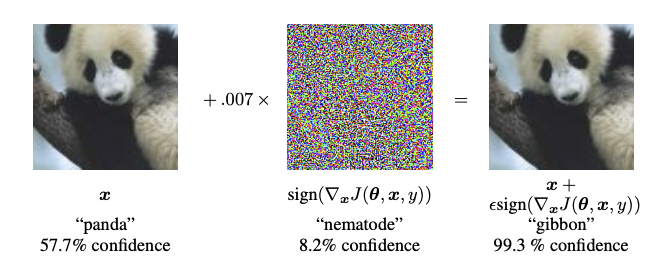
\includegraphics[width=10cm]{images/adversarial-example.png}
    \caption{Example of generating adversarial example with FSGM \cite{goodfellow2014explaining}}
\end{figure}

\textbf{FSGM}은 일반적인 이미지 $x$에 대해서 classifer의 decision boundary를 넘을 수 있는 노이즈가 섞인 adversarial example $x'$를 생성하는 것을 목표로 한다. 즉, 이것은 모델 파라미터 $\theta$, $x$ 에 대한 label $y$에 대해 loss $J(\theta, x, y)$를 최대화시키도록 학습시키는 것을 기본적인 골자로 adversarial example을 획득하는 것이다. 이때, 위에서 구한 loss를 곧바로 이용하는 것이 아니라, $x$에 대한 gradient인 $\nabla_x$를 loss에 곱하여 이미지의 각 픽셀이 loss에 기여하는 정도를 adversarial example에 반영할 수 있도록 하였다. 이를 수식으로 나타내면 아래와 같다. \cite{goodfellow2014explaining}

\[
x' = x + \epsilon \cdot \mathrm{sign}(\nabla_x J(\theta, x, y))
\] 


\subsubsection{PGD (Projected Gradient Descent)}

\textbf{PGD}는 FSGM과 같이 local maxima를 이용하여 adversarial example을 생성한다. 하지만, 기존 FSGM의 학습 과정을 $\alpha$ 의 크기에 따라 스텝으로 나누고, 그를 반복적으로 수행하여 더 좋은 결과를 이끌 수 있도록 FSGM보다 더 발전하였다. 이러한 PGD를 수식으로 나타내면 아래와 같다. \cite{madry2017towards}
\[
x^{t+1} = \Pi_{x + \mathcal{S}} (x^t + \alpha\mathrm{sign}(\nabla_x L(\theta, x, y)))
\]

\subsubsection{C\&W Attack}
C\&W는 어떤 이미지 $x$에 대해 classifier $C$ 가 잘못된 판단 $t$를 내리게 할 수 있는 최소한의 perturbation $\delta$를 생성하는 adversarial instance를 제안했다.\cite{carlini2017towards} 이 연구에서는 위 조건의 $\delta$를 생성하는 문제를 아래와 같은 문제로 모델링하였고, $f$가 될 수 있는 여러 함수에 대해 실험을 진행하여 최적인 함수를 채택하였다.

\[
\begin{array}{c}
    \textbf{minimize } ||\delta||_p + c \cdot f(x + \delta) \\
    \textbf{such that } x + \delta \in [0, 1]^n
\end{array}
\]

\subsection{기존 방어법}

\subsubsection{MagNet}

\begin{figure}[h]
    \centering
    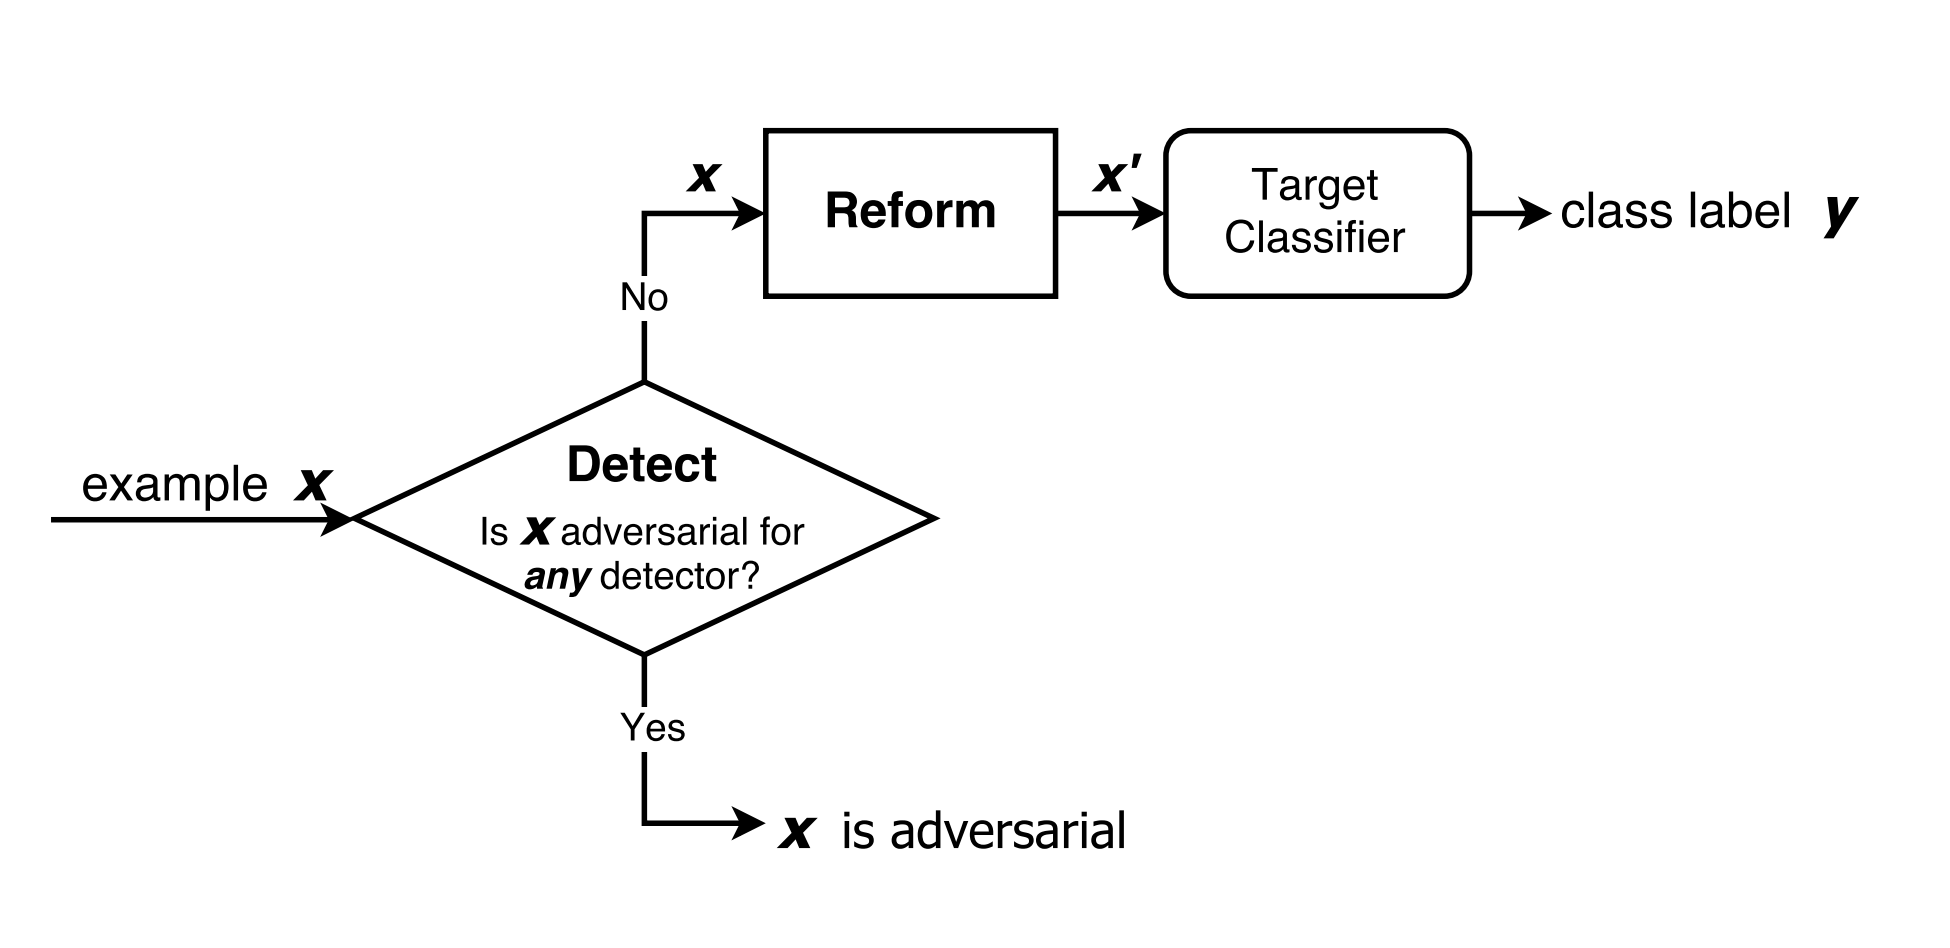
\includegraphics[width=10cm]{images/magnet-diagram.png}
    \caption{Two autoencoders of \textbf{MagNet} \cite{carlini2017magnet}}
\end{figure}

\textbf{MagNet}은 adversarial example을 이용한 공격을 효과적으로 방어하기 위해서 \textbf{Detector}와 \textbf{Reformer}를 활용한다.\cite{carlini2017magnet} Detector와 reformer는 둘 다 인공 신경망을 학습시킨 데이터를 통해 학습시킨 autoencoder들이다. Detector는 입력된 이미지와 출력된 이미지의 변화된 정도를 통해 해당 이미지가 adversarial example인지 아닌지 확인하는 장치이다. 두 이미지의 차이가 일정 임계 정도를 넘으면 adversarial example이라고 판단하는 방식이다. 그리고 reformer는 입력받은 이미지를 autoencoder를 통해 인공 신경망이 학습한 데이터에 더 가깝게 변환시키는 역할을 한다. 이를 통해 이미지에 섞인 perturbation을 제거하는 것을 목표로 한다. 하지만 detector의 존재 때문에 classifier의 기능성을 저해할 뿐만 아니라 \textbf{MagNet}이 방어에 별로 효과가 없다는 연구\cite{carlini2017magnet} 또한 존재한다.

\subsubsection{SHIELD}

\begin{figure}[h]
    \centering
    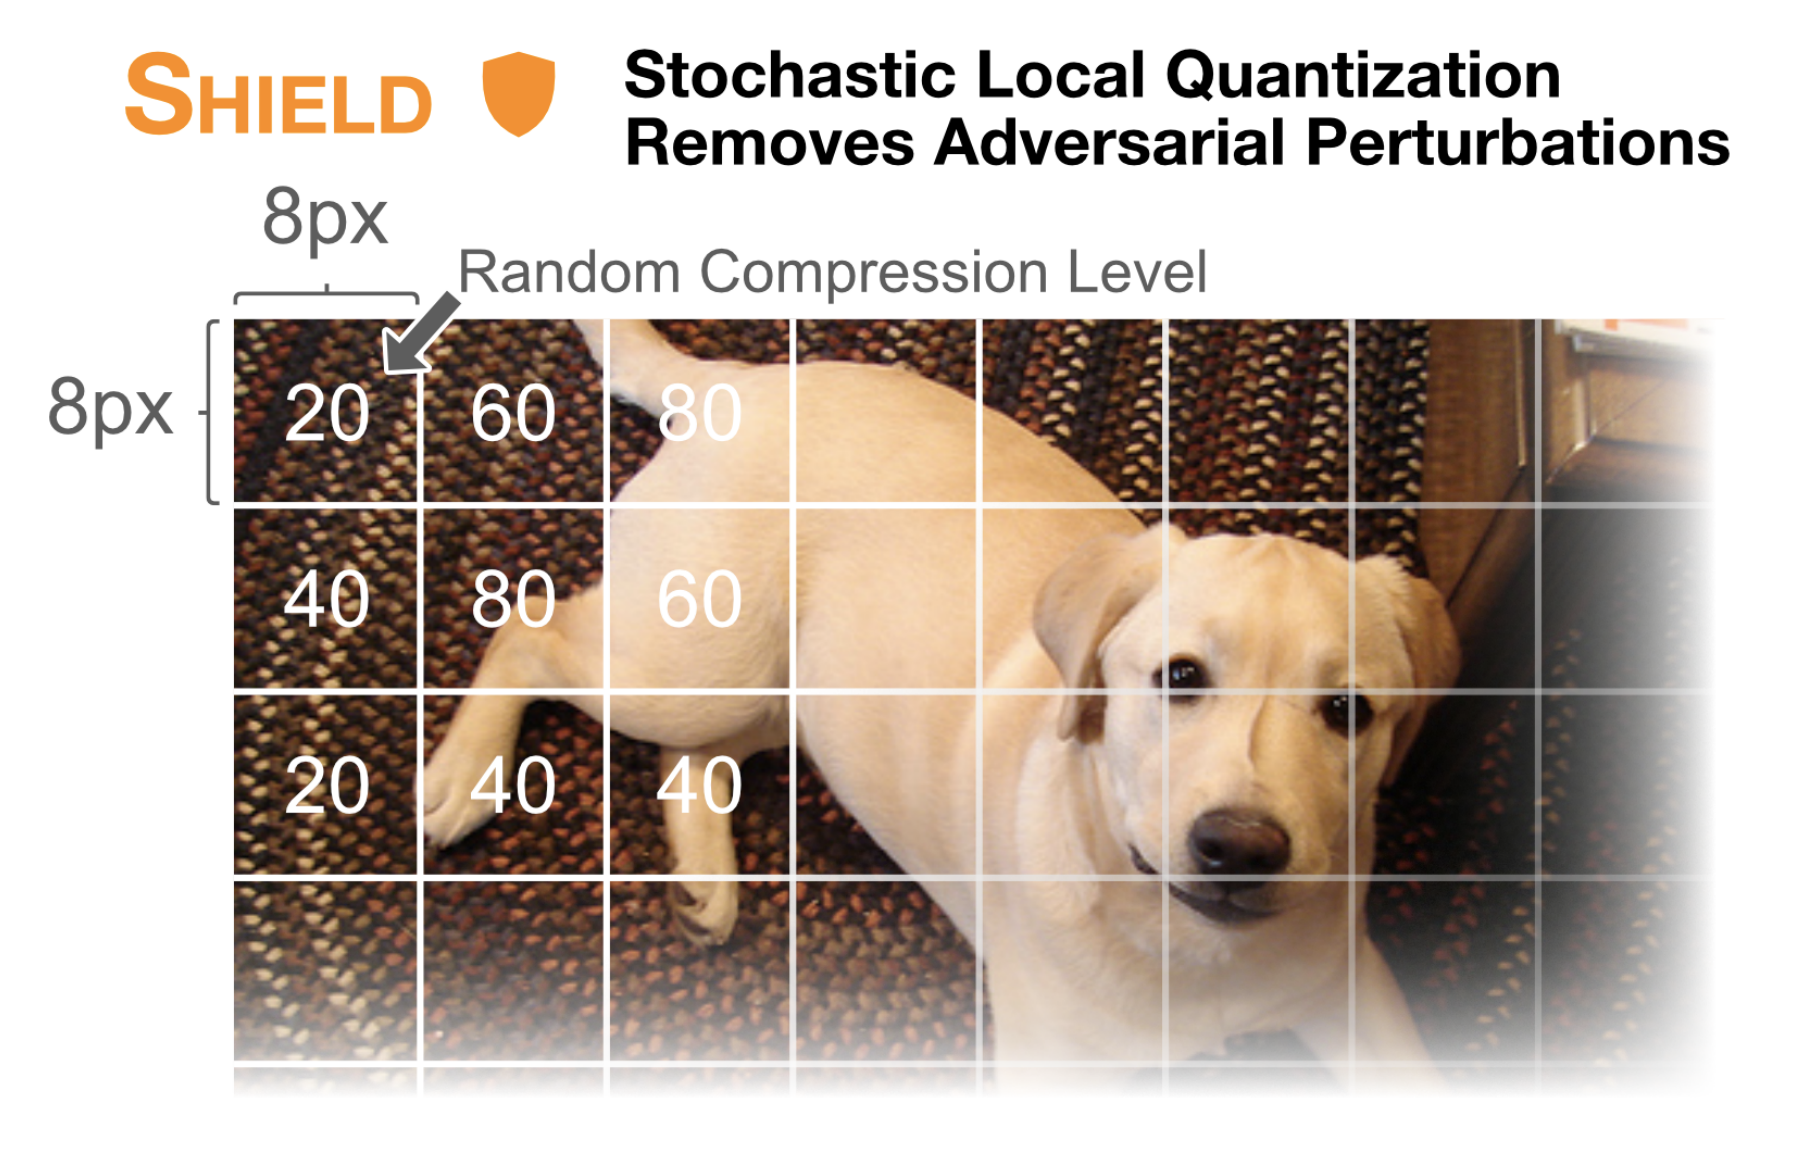
\includegraphics[width=8cm]{images/shield-example.png}
    \caption{Stochastic Local Quantization of \textbf{SHIELD} \cite{das2018shield}}
\end{figure}

\textbf{SHIELD}는 JPEG 압축을 통한 이미지 전처리를 통해 adversarial example의 perturbation을 제거하는 것을 목표로 하는 방어 체계이다.\cite{das2018shield} \textbf{SHIELD}는 공격을 효과적으로 방어하기 위해 SLQ (Stochastic Local Quantization) 이라고 이름 붙인 기술을 도입하였다. SLQ는 이미지를 그리드로 나누어서 각 칸을 랜덤의 압축률로 압축한 뒤 다시 하나의 이미지로 합치는 기술이다. 이 기술을 통해 perturbation을 최대한 억제할 수 있도록 만들었다고 연구진은 설명한다. 하지만 SLQ의 전처리 과정은 classfier를 오히려 방해하였고, 이를 해결하기 위해 연구진은 "vaccinate", 즉 기존 인공 신경망에 JPEG로 압축된 이미지를 추가적으로 학습시키는 과정을 거쳐야 했다. 압축을 통해 정보를 줄이는 의도는 좋았으나, SLQ의 압축 과정이 분류 체계을 방해하지 않도록 인공 신경망을 vaccinate해야한다는 점이 이식성을 저해하여 아쉽게 평가된다.

\subsubsection{Feature Distillation}
\textbf{Feature Distillation}은 기존 JPEG의 압축 과정을 개량하여 vaccinate 과정 없이 전처리할 수 있도록 함을 목표로 한다.\cite{liu2019feature} JPEG의 압축 과정은 사람의 눈에 보이기에 필요 없는 부분을 제거하는 것이지, 이것이 인공 신경망을 타겟팅했다고는 말하기 힘들다. 연구진은 이 특성을 이용하여, JPEG의 압축 과정에서 쓰이는 DCT와 양자화 과정을 인공 신경망에 맞게 개량하였고, 이를 통해 유의미한 이미지 전처리를 할 수 있었다.

\section{연구 방법}
%연구 수행 방법을 간략히 서술합니다.

\subsection{구현}

\begin{figure}[h]
    \centering
    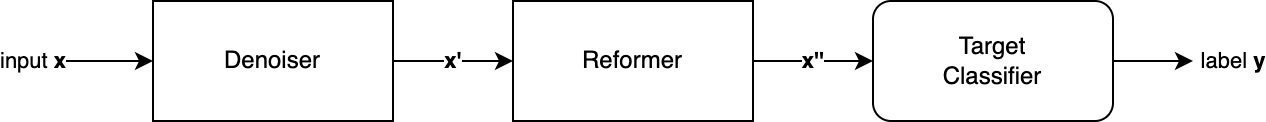
\includegraphics[width=10cm]{images/motd-diagram.png}
    \caption{Components of \textbf{MOTD}}
    \label{fig:motd-diagram}
\end{figure}

\textbf{MOTD}는 \textbf{SHIELD}의 압축 알고리즘을 수행하는 인스턴스인 denoiser과 \textbf{MagNet}의 refomer를 결합한 형태의 시스템으로, 방어 체계의 이식성을 높이는 동시에 인공 신경망의 기능성을 저해하지 않는 모듈형 sanitizer를 목표로 한다. \textbf{MOTD}의 파이프라인은 Figure \ref{fig:motd-diagram}와 같다. \textbf{MOTD}에 입력된 이미지는 우선 \cite{das2018shield}에 제시된 SLQ (Stochastic Local Quantization) 알고리즘을 통해 전처리되며, 이 전처리된 이미지는 reformer를 거치면서 vaccinate 되지 않은 인공 신경망이 분류할 수 있는 형태로 가공된다.

\subsection{평가 방법}

\textbf{MOTD}의 성능 평가를 위해서 타겟이 될 인공 신경망과 위협 모델이 필요하다. 타겟이 될 인공 신경망으로는 MNIST를 분류하는 인공 신경망과 CIFAR-10을 분류하는 인공 신경망을 채택할 것이다. 범용적으로 실험에 많이 이용되는 데이터셋임을 고려하여, 이들을 분류하는 인공 신경망을 공격 대상으로 채택하였다. 그리고, 이들을 공격하는 위협 모델으로는 FSGM, PGD, 그리고 C\&W attack의 구현체를 채택할 것이다. 셋의 공격 방법이 classifier의 공격에 널리 사용됨을 고려하여 셋의 공격에 대해 \textbf{MOTD}가 얼마나 잘 방어할 수 있을지 측정할 것이다.

\textbf{MOTD}를 본격적으로 평가하기 이전에, detector가 시스템의 기능성 저하에 얼마나 기여하는지 살펴보기 위해 detector에서 adversarial example이라고 판단된 이미지들에 대해서 인공 신경망이 올바른 판단을 내릴 수 있는지 확인해볼 것이다. 이후에, 위의 조건 하에서 detector를 제거한 \textbf{MagNet}, vaccinate 되지 않은 인공 신경망에 대한 \textbf{SHIELD}, \textbf{MagNet}, 그리고 \textbf{SHIELD}와 \textbf{MOTD}의 방어 성능을 비교할 것이다. 앞선 두 조건의 데이터를 통해 둘이 결합된 형태인 \textbf{MOTD}가 실질적으로 성능이 향상되었는지 보일 것이며, 정상적인 조건의 \textbf{MagNet}, \textbf{SHIELD}와의 비교를 통해 실질적으로 방어를 해낼 수 있을지 그 여부를 보일 것이다.  

\section{기대 효과}
%연구 결과를 통해 기대할 수 있는 학계 또는 산업계의 파급 효과를 간략히 서술합니다. 

\textbf{MagNet}은 2단계의 파이프라인을 통해 효율적이면서도 이식성 높은 방어 방법을 제시했다고 볼 수 있으나, detector의 존재는 인공 신경망의 기능성을 저해하는 역할을 수행했다고 볼 수 있다. 예를 들어, 방어 체계가 해당 이미지를 올바르게 전처리 했다면 인공 신경망이 제 역할을 수행할 수 있었을 뿐만 아니라, 전처리 없이도 인공 신경망이 충분히 판단할 수 있는 이미지를 detector가 기각하는 경우가 있을 수 있기 때문이다. 이러한 관점에서, \textbf{MOTD}는 dectector 제거를 통해 위양성 리스크를 제거하여 전체 시스템의 기능성을 높일 수 있다. 또한, \textbf{SHIELD}의 경우 효율적인 압축 알고리즘을 이용하여 빠른 전처리 성능을 보였으나 이를 이용하기 위해서는 인공 신경망에 압축된 형태의 이미지들을 미리 학습시켜야 한다는 치명적인 단점을 가지고 있다. \textbf{MOTD}는 \textbf{SHIELD}의 전처리 이후 해당 이미지를 reformer로 처리하여 vaccination 없이 전처리된 이미지를 바로 이용할 수 있도록 만들어 방어 체계의 이식성을 높일 수 있다. 즉, \textbf{MOTD}는 전체 시스템의 기능성을 저해시키지 않는 동시에 이식성이 높은 방어 체계이며, 이를 통해 인공 신경망 파이프라인의 적재적소에 추가될 수 있는 모듈형 방어 체계를 제시하고자 한다. 


\section{연구 추진 일정}
%최종 발표에 맞추어 개략적인 연구 추진 계획을 기록합니다.

해당 연구를 수월하게 수행하기 위해서 아래 표와 같은 일정을 수립하였다. 

\begin{table}[h]
    \centering
    \label{t2}
    \begin{tabular}{c|c}
        \noalign{\smallskip}\noalign{\smallskip}\hline
        2022. 03. 11. & 연구 제안서 제출  \\
        \hline
        2022. 03. 21. & 보호하고자 하는 인공 신경망 모델 생성 \\
        \hline
        2022. 03. 31. & Dectector의 위양성 리스크 측정 \\
        \hline
        2022. 04. 11. & Detector가 제거된 \textbf{MagNet}과 vaccination 없는 \textbf{SHIELD}에 대한 성능 평가 \\
        \hline
        2022. 04. 22. & 연구 진행 보고서 제출  \\
        \hline
        2022. 05. 11. & \textbf{MOTD} 구현 \\
        \hline
        2022. 05. 20. & 타 방어 기법과 비교 및 평가 \\
        \hline
        2022. 06. 01. & 연구 결과 보고서 제출  \\
        \hline
    \end{tabular}
\end{table}

\bibliographystyle{plain}
\bibliography{references}
\end{document}
